% !TeX root = Microwave.tex
\chapter{天线的电参数}
\begin{equation*}
\mbox{天线参数}
\begin{cases}
    \mbox{电路参量}
    \begin{cases}
        \mbox{天线阻抗}\\
        \mbox{辐射电阻}
    \end{cases}\\
    \mbox{空间参量}
    \begin{cases}
        \mbox{场波瓣图}\\
        \mbox{功率波瓣图}\\
        \mbox{定向性}D\\
        \mbox{增益}G\\
        \mbox{极化}\mathrm{LP},\mathrm{CP},\mathrm{EP}
    \end{cases}
\end{cases}
\end{equation*}

\section{辐射特性参数}
    辐射特性有功率通量密度$\vec{S}(\theta,\phi)$(Power flux density)、辐射强度$P_r(\theta,\phi)$(Radiation intensity)、场强(Fields strength)、相位(Phase)、极化(Polarization)等;

    \subsection{辐射方向图}
    天线的辐射方向图一般描述天线在远场区的辐射特性。
    \begin{definition}{辐射方向图(Radiation Pattern)}{辐射方向图}
    天线的辐射特性是关于空间坐标的函数,若在\textbf{固定距离}上,此函数通过数学函数或者图形来描述,则得到的数学函数或者图形即为辐射方向图(Radiation Pattern),简称方向图。
    \tcblower
    通常而言,这里的辐射特性指电场强度,空间坐标表示为$(\theta,\phi)$。则天线的方向图定义为
    \begin{equation}
        f(\theta,\phi)=\frac{|\vec{E}(\theta,\phi)|}{A_0}
    \end{equation}
    其中$A_0$是$|\vec{E}(\theta,\phi)|$表达式中与$\theta,\phi$无关的因式。
    
    这种定义又叫 Field Amplitude Pattern,区别于 Power Pattern。
    \end{definition}    
    

    \begin{corollary}{归一化方向图}{归一化方向图}
        定义天线的归一化场强方向图为$F(\theta,\phi)$:
        \begin{equation}
            F(\theta,\phi)
            =\frac{f(\theta,\phi)}{f_\mathrm{max}}
            =\frac{|E(\theta,\phi)|}{E_\mathrm{m}}
        \end{equation}
        则天线的归一化功率方向图可以表示为$F^2(\theta,\phi)$。
    \end{corollary}


        
        方向图中主要关注的参数:
        \begin{enumerate}
            \item 零功率波瓣宽度(FNBW) $2\theta_{OE}$ 和 $2\theta_{OH}$:指主瓣最大值两边两个零辐射方向的夹角。
            \item 半功率波瓣宽度(HPBW) $2\theta_{OE}$ 和 $2\theta_{OE}$:指主瓣最大值两边功率通量密度下降到最大值的一半(或场强下降到最大值的0.707)时,即下降\SI{3}{\decibel}的两点间的夹角。
            \item 旁瓣电平(FSLL):指第一旁瓣功率密度和主瓣功率密度之比的对数值
                \begin{equation}
                    \xi_1=10\lg\frac{S(\theta_1,\varphi_1)}{S} 
                \end{equation}
            副瓣方向通常是不需要辐射或接收能量的方向。因此,天线副瓣电平越低,表明天线在不需要方向上辐射或接收的能量越弱,或者说在这些方向上对杂散的来波抑制能力越强,抗干扰能力就越强。因此,在天线设计中常有低副瓣设计要求。如基站的上旁瓣、雷达天线。
            
            \item 前后抑制比 $\xi_b$:后瓣最大辐射方向上功率密度和主瓣功率密度之比的对数值。
                \begin{equation}
                    \xi_b=10\lg\frac{S_b}{S_M}=20\lg\frac{|E_b|}{|E_M|}
                \end{equation}
        \end{enumerate}

        \begin{figure}[htp]
            \centering
            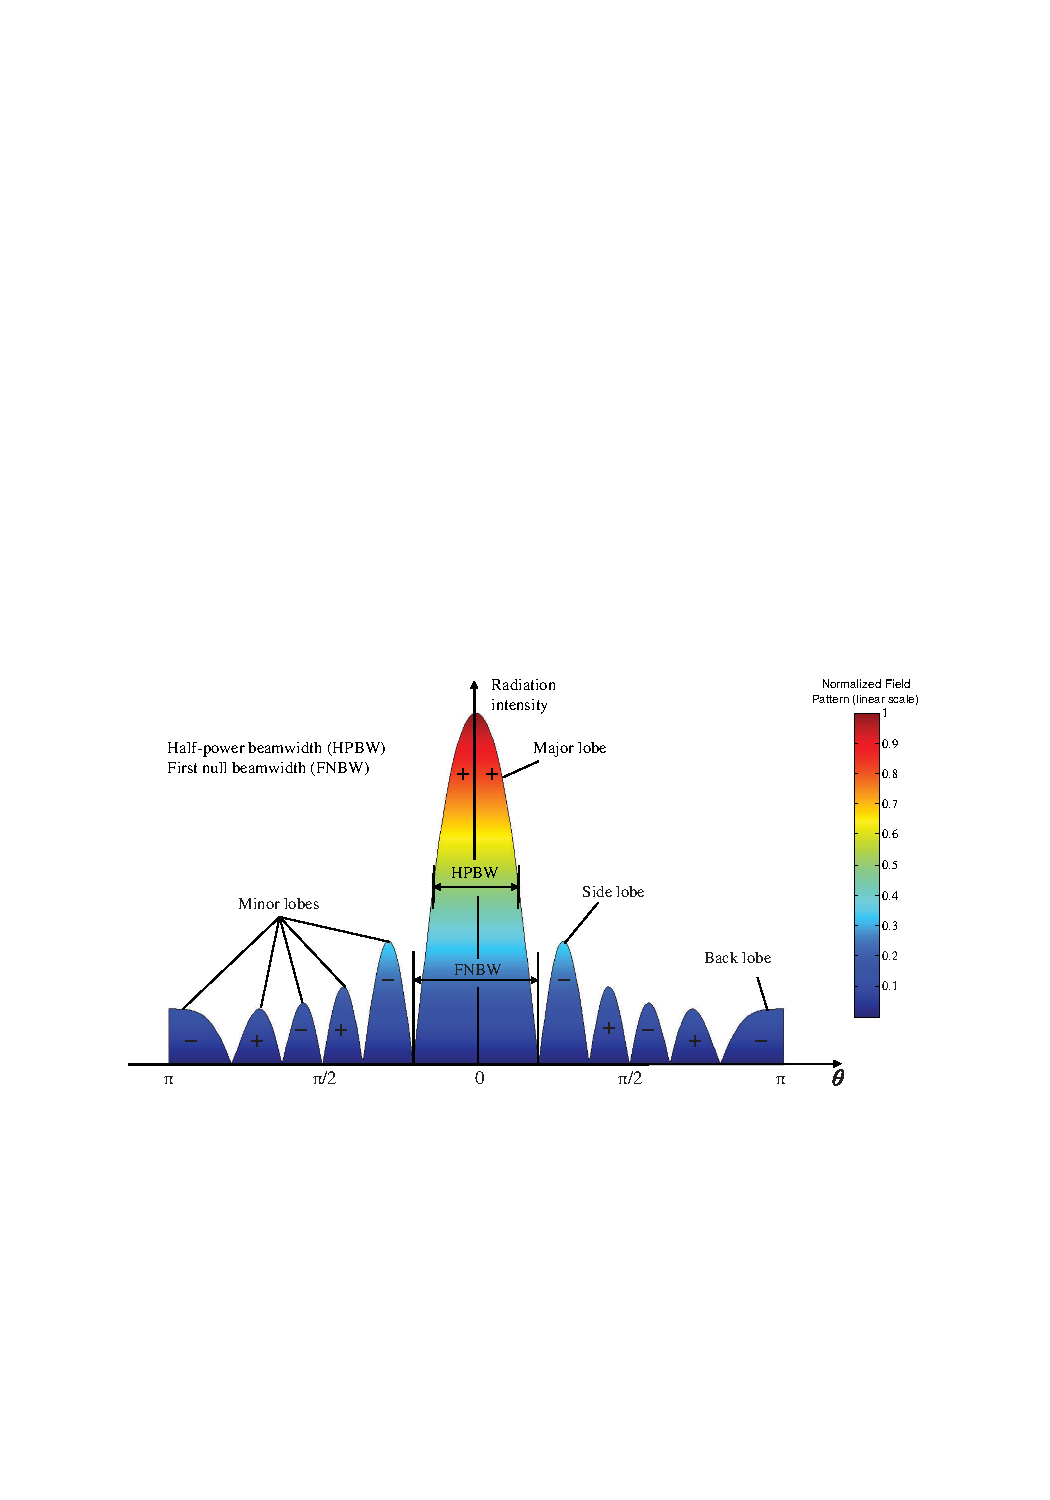
\includegraphics[width=14cm]{figure/5-2.pdf}
            \caption{\kaishu 某直角坐标下的功率方向图}\label{Fig: 天线方向图图例}
        \end{figure}

    \subsection{对称振子的辐射场}
        求解将对称振子分为许多小段,则每一小段都可看做一电基本振子,对于线性媒质,应用叠加原理,则对称振子的辐射场就等于这些无数小段基本振子辐射场的叠加。
        对称振子的电流分布近似为

        式中α:振子电流的相移常数。
        如果不考虑振子电流由辐射引起的
        衰减,忽略振子粗细的影响

    \subsection{辐射功率和辐射电阻}
        天线的输入功率一般为复功率,根据玻印廷定理,取包围天线所在体积$V$的任意封闭面$S$
        \begin{equation}
            \dot{p}_A=p_l+\dot{p}_\Sigma
        \end{equation}

        $V$内的损耗功率(导体损耗和介质损耗)
        \begin{equation}
            p_l=
        \end{equation}
        天线的全辐射功率
        =R+j2
        ='Reg,(E×H')-d.
        天线的辐射功率
        f
        辐射的无功功率
        =士1m)手,(E×H )-ask
        +j2o(Wm一WR)


        辐射功率与线天线上电流的大小有关,不便于直接比较天线的性能。为此引入天线的辐射阻抗概念。假设天线的全辐射功率被一个等效阻抗所“吸收”,该阻抗上流过的电流为天线上某处的电流,称此等效阻抗为天线的辐射阻抗。如天线上某处电流的振幅为I,则辐射阻抗
        \begin{equation}
            Z_\Sigma=\frac{P_\Sigma+\mathrm{j}Q_\Sigma}{\frac{1}{2}I^2}=R_\Sigma+\mathrm{j}X_\Sigma
        \end{equation}

        使用 波腹电流$I_M$ 或 输入电流$I_A$ 来计算,可以得到不同意义下的辐射阻抗$Z_\Sigma$和$Z_{\Sigma A}$,
        两种阻抗值不同,但满足
        
        \begin{equation}
            \frac{1}{2}=
        \end{equation}

        采用玻印廷矢量法计算天线的实辐射功率(以后简称辐射功率)和辐射电阻。

    \subsection{辐射功率和辐射阻抗}

        \begin{equation*}
        \mbox{计算辐射功率和辐射阻抗}
        \begin{cases}
            \mbox{远场区——Poynting矢量法,辐射实功率,辐射电阻}\\
            \mbox{近场区——感应电势法,复功率,辐射电阻和电抗}
        \end{cases}
        \end{equation*}

        远场区辐射功率
        \begin{equation}
            P_\Sigma=\frac{1}{120\pi}
        \end{equation}

        辐射电阻
        \begin{equation}
            R_\Sigma=\frac{2P_\Sigma}{|I_M|^2}=60 \int_{0}^{\pi}\frac{[]^2}{\sin\theta}\,\mathrm{d}\theta
        \end{equation}

    \subsection{天线的有效长度}
    \subsection{方向系数}
        天线的方向系数:用数字定量地表示辐射电磁能量集束程度,描述天线的方向特性数,又叫做方向性系数或方向性增益。
        
        
        \begin{definition}{辐射功率}{辐射功率}
            设有一球面$S$,半径为$r$,球心位于天线中心。天线的辐射功率,定义为\textbf{天线辐射场穿过球面$S$的功率}:
            \begin{equation}
                P_r(\vec{r})
                =\oint_S \vec{S}_r\cdot\mathrm{d}\vec{S}
            \end{equation}
        \end{definition}

        \begin{definition}{辐射强度}{辐射强度}
            天线在某方向的辐射强度,定义为\textbf{该方向上单位立体角内的辐射功率}:
            \begin{equation}
                U(\theta,\varphi)=
            \end{equation}
        \end{definition}

        \begin{definition}{方向系数}{方向系数}
            天线在某方向的方向系数$D(\theta,\varphi)$是该方向上的辐射强度$U(\theta,\varphi)$与平均辐射强度之比,平均辐射强度为$\frac{1}{4}$,即
            \begin{equation}
                D(\theta,\varphi)=\frac{4\pi F^2(\theta,\varphi)}{\int_{0}^{2\pi}\int_{0}^{\pi}F^2(\theta,\varphi)\sin\theta\,\mathrm{d}\theta\mathrm{d}\varphi}
            \end{equation}

            最大辐射方向的方向系数:某天线的方向系数通常均指最大辐射方向的方向系数。

        \end{definition}

        \begin{definition}{天线增益}{天线增益}
            天线的在某方向的增益$G(\theta,\varphi)$是该方向辐射强度$U(\theta,\varphi)$同天线 \underline{以同一输入功率} 向空间均匀辐射的辐射强度$\dfrac{P_A}{4\pi}$之比,即
            \begin{equation}
                G(\theta,\varphi)=4\pi \frac{U(\theta,\varphi)}{P_A}
            \end{equation}

            增益与方向系数的关系
            \begin{equation}
                G(\theta,\varphi)=D(\theta,\varphi)\eta_A
            \end{equation}

            某天线的增益通常指最大辐射方向增益:
            \begin{equation}
                G=4\pi \frac{U_M}{P_A}=D_M\eta_A
            \end{equation}
        \end{definition}

        
    \subsection{对称振子的输入阻抗}
    
\section{的}
